\chapter{控制系统数学模型}

\intro{建立被控对象的数学模型是控制系统分析与设计的第一步。本章系统介绍微分方程建模、传递函数建立、框图化简与信号流图方法。}

\section{微分方程建模}

描述物理系统的数学模型通常是一组微分方程。以下通过几个典型实例说明从物理定律到微分方程的建模过程。

\subsection{RLC电路}

\begin{figure}[H]
\centering
\begin{tikzpicture}[
    ctrlCirc/.style={thick},
    ctrlLabelC/.style={font=\footnotesize},
]
% RLC series circuit
\draw[ctrlCirc] (0,0) to[V, l=$e_i(t)$] (0,3);
\draw[ctrlCirc] (0,3) to[R, l=$R$] (3,3);
\draw[ctrlCirc] (3,3) to[L, l=$L$] (5,3);
\draw[ctrlCirc] (5,3) to[C, l=$C$] (5,0);
\draw[ctrlCirc] (5,0) -- (0,0);
% Current arrow and output voltage
\draw[ctrlCirc,->] (1.0,2.6) -- (1.8,2.6) node[above,ctrlLabelC] {$i(t)$};
\draw[ctrlCirc,->] (5.5,1.5) -- (6.5,1.5) node[above,ctrlLabelC] {$e_o(t)$};
\node[font=\footnotesize] at (2.5,-0.6) {$e_o(t) = \frac{1}{C}\int i(t)dt$};
\end{tikzpicture}
\caption{RLC串联电路}
\label{fig:rlc-circuit}
\end{figure}

由Kirchhoff电压定律：
\[
e_i(t) = Ri(t) + L\frac{di}{dt} + \frac{1}{C}\int i(t)\,dt
\]
输出为电容电压：$e_o(t) = \frac{1}{C}\int i(t)dt$。代入$i = C\dot{e}_o$，得到：
\[
LC\frac{d^2e_o}{dt^2} + RC\frac{de_o}{dt} + e_o = e_i
\]

这是典型的二阶线性ODE。物理参数$L'$（电感）、$R$（电阻）、$C$（电容）直接决定了系统的动态行为。标准化形式：
\[
\ddot{e}_o + 2\zeta\omega_n \dot{e}_o + \omega_n^2 e_o = \omega_n^2 e_i
\]
其中自然频率$\omega_n = 1/\sqrt{LC}$，阻尼比$\zeta = \frac{R}{2}\sqrt{C/L}$。

取Laplace变换（零初始条件）得传递函数：
\[
G(s) = \frac{E_o(s)}{E_i(s)} = \frac{1}{LC s^2 + RCs + 1} = \frac{\omega_n^2}{s^2 + 2\zeta\omega_n s + \omega_n^2}
\]

\subsection{质量-弹簧-阻尼系统}

\begin{figure}[H]
\centering
\begin{tikzpicture}[
    ctrlMech/.style={thick},
    ctrlLabelM/.style={font=\footnotesize},
]
% Wall
\draw[ctrlMech, fill=gray!30] (-0.2, -0.8) rectangle (0, 3.8);
\draw[ctrlMech, pattern=north east lines] (-0.2, -0.8) rectangle (0, 3.8);
% Spring
\draw[ctrlMech, decorate, decoration={coil, aspect=0.6, segment length=4pt, amplitude=4pt}] (0,2.5) -- (2.5,2.5);
\node[ctrlLabelM] at (1.25, 2.0) {$k$};
% Mass
\draw[ctrlMech, fill=blue!20] (2.5,1.8) rectangle (4.2,3.2);
\node[ctrlLabelM] at (3.35,2.5) {$m$};
% Damper
\draw[ctrlMech] (4.2,3.0) -- (5.5,2.5);
\draw[ctrlMech] (4.2,2.0) -- (5.5,1.5);
\draw[ctrlMech, fill=gray!20] (5.5,1.3) rectangle (6.2,2.7);
\node[ctrlLabelM] at (5.85, 2.0) {$b$};
% Fixed point for damper
\draw[ctrlMech, fill=gray!30] (6.2, 1.3) rectangle (6.5, 2.7);
\draw[ctrlMech, pattern=north east lines] (6.2, 1.3) rectangle (6.5, 2.7);
% Force arrow
\draw[ctrlMech, ->] (3.35, 3.8) -- (3.35,3.4);
\node[ctrlLabelM] at (3.35, 4.0) {$f(t)$};
% Ground
\draw[ctrlMech] (-0.5, -0.8) -- (7.0,-0.8);
% Displacement label
\draw[ctrlMech, ->] (3.35, -0.3) -- (3.35, 0.3);
\node[ctrlLabelM] at (4.0, 0.0) {$y(t)$};
\end{tikzpicture}
\caption{质量-弹簧-阻尼机械系统}
\label{fig:mass-spring-damper}
\end{figure}

由Newton第二定律，受力分析：
\[
f(t) - b\frac{dy}{dt} - ky = m\frac{d^2y}{dt^2}
\]
整理得：
\[
m\ddot{y} + b\dot{y} + ky = f(t)
\]
标准化为：
\[
\ddot{y} + \frac{b}{m}\dot{y} + \frac{k}{m}y = \frac{1}{m}f(t)
\]

取Laplace变换得：
\[
G(s) = \frac{Y(s)}{F(s)} = \frac{1}{ms^2 + bs + k} = \frac{1/m}{s^2 + (b/m)s + k/m}
\]

自然频率$\omega_n = \sqrt{k/m}$，阻尼比$\zeta = \frac{b}{2\sqrt{mk}}$。值得注意的是，RLC电路和质量-弹簧-阻尼系统具有\textbf{完全相同的数学结构}——这是物理系统之间的"对偶性"（duality），揭示了不同工程领域背后的统一数学框架。

\subsection{直流电机}

电枢控制的直流电机的动态方程为：
\[
\begin{cases}
L_a \frac{di_a}{dt} + R_a i_a + K_b \dot{\theta} = e_a(t) & \text{（电枢回路）}\\[4pt]
J \ddot{\theta} + b \dot{\theta} = K_t i_a & \text{（机械负载）}
\end{cases}
\]
其中$e_a$为电枢电压（输入），$\theta$为转角（输出），$K_b$为反电动势系数，$K_t$为转矩系数。

忽略电感$L_a$（对多数电机近似成立）时，消去$i_a$可得：
\[
J \ddot{\theta} + \left(b + \frac{K_b K_t}{R_a}\right)\dot{\theta} = \frac{K_t}{R_a} e_a
\]

传递函数为：
\[
G(s) = \frac{\Theta(s)}{E_a(s)} = \frac{K_m}{s(\tau_m s + 1)}
\]
其中电机增益$K_m = K_t/(R_a b + K_b K_t)$，机电时间常数$\tau_m = JR_a/(R_a b + K_b K_t)$。

\begin{figure}[H]
\centering
\begin{tikzpicture}[
    ctrlStep/.style={rectangle,draw=black,fill=blue!15,minimum width=2.8cm,minimum height=0.9cm,font=\footnotesize,align=center},
    ctrlArrowR/.style={->,>=stealth,thick},
]
\node[ctrlStep] at (0,0) {物理系统\\（RLC/机械/电机）};
\node[ctrlStep] at (4,0) {微分方程\\$a_n y^{(n)}+\cdots+a_0 y = b_m u^{(m)}+\cdots+b_0 u$};
\node[ctrlStep] at (8,0) {传递函数\\$G(s)=Y(s)/U(s)$};
\node[ctrlStep] at (12,0) {框图模型};
\draw[ctrlArrowR] (1.7,0) -- (2.3,0) node[midway,above,font=\footnotesize] {物理定律};
\draw[ctrlArrowR] (5.7,0) -- (6.3,0) node[midway,above,font=\footnotesize] {Laplace变换};
\draw[ctrlArrowR] (9.7,0) -- (10.3,0) node[midway,above,font=\footnotesize] {结构图};
\end{tikzpicture}
\caption{从物理系统到数学模型的一般建模流程}
\label{fig:modeling-flow}
\end{figure}

\begin{remark}
以上三个实例——RLC电路、质量-弹簧-阻尼系统和直流电机——分别代表了电气、机械和机电三类对象。它们的建模过程遵循统一范式：物理定律→微分方程→Laplace变换→传递函数。这一范式贯穿整个经典控制理论。
\end{remark}

\section{传递函数与典型环节}

\subsection{典型环节的传递函数}

任何复杂的线性系统均可分解为以下几种基本环节的串联或并联组合：

\begin{enumerate}
\item \textbf{比例环节}（Proportional）：$G(s) = K$。
其输出与输入成正比，无时间延迟。例如理想放大器、杠杆机构。阶跃响应为幅度$K$的阶跃。

\item \textbf{积分环节}（Integral）：$G(s) = 1/s$。
输出为输入的积分。阶跃响应为斜率等于1的斜坡信号。积分环节具有"记忆"功能，能消除稳态误差，但会引入$-90^\circ$的相位滞后。

\item \textbf{微分环节}（Derivative）：$G(s) = s$。
输出为输入的微分。理想微分环节在物理上不可实现（分子阶次高于分母），实际中使用带滤波的近似微分环节。

\item \textbf{惯性环节}（First-order lag）：$G(s) = \frac{K}{Ts+1}$。
一阶滞后环节，时间常数$T$反映响应速度。阶跃响应为$y(t) = K(1-e^{-t/T})$。

\item \textbf{振荡环节}（Second-order oscillation）：$G(s) = \frac{\omega_n^2}{s^2 + 2\zeta\omega_n s + \omega_n^2}$。
当$0 < \zeta < 1$时，阶跃响应为衰减振荡；$\zeta \geq 1$时为无超调单调过程。

\item \textbf{纯滞后环节}（Time delay）：$G(s) = e^{-\tau s}$。
输出无畸变地滞后输入$\tau$秒。在频域中滞后环节对相位的影响极大，是反馈系统设计中的不利因素。
\end{enumerate}

\begin{myformula}
\textbf{六种典型环节的传递函数汇总：}\\[\medskipamount]
\text{比例:}&\quad G(s)=K \notag\\
\text{积分:}&\quad G(s)=\frac{1}{s} \notag\\
\text{理想微分:}&\quad G(s)=s \notag\\
\text{惯性:}&\quad G(s)=\frac{K}{Ts+1} \notag\\
\text{振荡:}&\quad G(s)=\frac{\omega_n^2}{s^2+2\zeta\omega_n s+\omega_n^2} \notag\\
\text{纯滞后:}&\quad G(s)=e^{-\tau s} \notag
\end{myformula}

\section{框图及其化简}

\subsection{方框图的基本连接方式}

控制系统的功能框图由方框、信号线、比较点和引出点四种基本元素组成。多个环节之间有三种基本连接方式：

\subsubsection*{串联连接}
$n$个环节串联时，总传递函数为各环节传递函数的乘积：
\[
G(s) = G_1(s)G_2(s)\cdots G_n(s)
\]

\subsubsection*{并联连接}
$n$个环节并联时，总传递函数为各环节传递函数之和：
\[
G(s) = G_1(s) + G_2(s) + \cdots + G_n(s)
\]

\subsubsection*{反馈连接}
前向通道$G(s)$与反馈通道$H(s)$构成的闭环传递函数为：
\[
\Phi(s) = \frac{Y(s)}{R(s)} = \frac{G(s)}{1 + G(s)H(s)}
\]
分母中"$+$"对应负反馈（比较点处为减号），"$-$"对应正反馈。

\begin{proof}[负反馈闭环传函推导]
由框图：$E(s) = R(s) - B(s)$，$B(s) = H(s)Y(s)$，$Y(s) = G(s)E(s)$。消去$E(s)$和$B(s)$：
\[
Y(s) = G(s)[R(s)-H(s)Y(s)] = G(s)R(s) - G(s)H(s)Y(s)
\]
移项：
\[
[1 + G(s)H(s)]Y(s) = G(s)R(s) \quad\Rightarrow\quad \Phi(s) = \frac{G(s)}{1+G(s)H(s)}
\]
\end{proof}

\subsection{框图等效变换规则}

典型的框图化简遵循以下六条等价规则（表\ref{tab:block-rules}）。

\begin{table}[H]
\centering
\caption{框图等效变换规则}
\label{tab:block-rules}
\renewcommand{\arraystretch}{1.6}
\begin{tabular}{|c|p{4.5cm}|p{4.5cm}|}
\hline
\textbf{序号} & \textbf{原框图} & \textbf{等效框图} \\
\hline
1（比较点前移） &
比较点从环节前移至环节后：在反馈通道中串联该环节 &
比较点从环节后移至环节前：在反馈通道中串联该环节的倒数 \\
\hline
2（引出点前移） &
引出点从环节后移至环节前：引出通道中串联该环节 &
引出点从环节前移至环节后：引出通道中串联该环节的倒数 \\
\hline
3（串联化简） &
$R \rightarrow [G_1] \rightarrow [G_2] \rightarrow Y$ &
$R \rightarrow [G_1G_2] \rightarrow Y$ \\
\hline
4（并联化简） &
$R \rightarrow \begin{matrix} [G_1] \\ [G_2] \end{matrix} \rightarrow \oplus \rightarrow Y$ &
$R \rightarrow [G_1+G_2] \rightarrow Y$ \\
\hline
5（反馈化简） &
前向$G$，反馈$H$，比较点（减号） &
$R \rightarrow [\frac{G}{1+GH}] \rightarrow Y$ \\
\hline
6（单位反馈化） &
非单位反馈$\Phi = \frac{G}{1+GH}$ &
等价为单位反馈右乘$1/H$：或变换为$\frac{G}{1+GH} = \frac{1}{H}\cdot\frac{GH}{1+GH}$ \\
\hline
\end{tabular}
\end{table}

框图化简的基本策略是：逐步移动比较点和引出点，消除交叉耦合，将内环化简，最终得到单一传递函数。

\begin{example}
化简图\ref{fig:block-reduction}所示的多回路系统。

\begin{figure}[H]
\centering
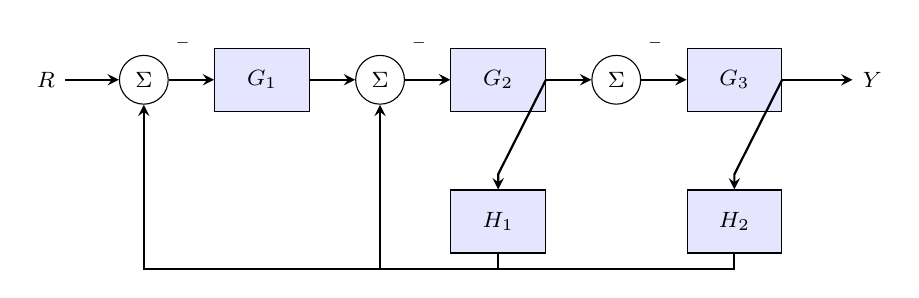
\begin{tikzpicture}[
    ctrlBk/.style={rectangle,draw=black,fill=blue!10,minimum width=1.2cm,minimum height=0.8cm,font=\footnotesize},
    ctrlSm/.style={circle,draw=black,minimum size=0.5cm,font=\footnotesize\bfseries},
    ctrlArr/.style={->,>=stealth,thick},
]
\node[ctrlBk] (G1) at (2.0,0) {$G_1$};
\node[ctrlBk] (G2) at (5.0,0) {$G_2$};
\node[ctrlBk] (G3) at (8.0,0) {$G_3$};
\node[ctrlBk] (H1) at (5.0,-1.8) {$H_1$};
\node[ctrlBk] (H2) at (8.0,-1.8) {$H_2$};
\node[ctrlSm] (S1) at (0.5,0) {$\Sigma$};
\node at (S1.north east)[above right=0.05cm,font=\tiny] {$-$};
\node[ctrlSm] (S2) at (3.5,0) {$\Sigma$};
\node at (S2.north east)[above right=0.05cm,font=\tiny] {$-$};
\node[ctrlSm] (S3) at (6.5,0) {$\Sigma$};
\node at (S3.north east)[above right=0.05cm,font=\tiny] {$-$};
\draw[ctrlArr] (-0.5,0) node[left,font=\footnotesize] {$R$} -- (S1);
\draw[ctrlArr] (S1) -- (G1);
\draw[ctrlArr] (G1) -- (S2);
\draw[ctrlArr] (S2) -- (G2);
\draw[ctrlArr] (G2) -- (S3);
\draw[ctrlArr] (S3) -- (G3);
\draw[ctrlArr] (G3.east) -- (9.5,0) node[right,font=\footnotesize] {$Y$};
% Feedback paths
\draw[ctrlArr] (G2.east) -- (5.0,-1.2) -- (H1.north);
\draw[ctrlArr] (H1.south) -- (5.0,-2.4) -- (0.5,-2.4) -- (S1.south);
\draw[ctrlArr] (G3.east) -- (8.0,-1.2) -- (H2.north);
\draw[ctrlArr] (H2.south) -- (8.0,-2.4) -- (3.5,-2.4) -- (S2.south);
\end{tikzpicture}
\caption{多回路控制系统框图}
\label{fig:block-reduction}
\end{figure}

{\heiti 解}：从最内环开始化简。内环1（$H_2$反馈环）：
\[
G_{23,\text{eq}} = \frac{G_2}{1+G_2G_3H_2}
\]
化简后，外环变为$H_1$的反馈环，前向通道为$G_1 G_{23,\text{eq}} G_3$：
\[
\Phi(s) = \frac{G_1 \cdot \frac{G_2}{1+G_2G_3H_2} \cdot G_3}{1 + G_1 \cdot \frac{G_2}{1+G_2G_3H_2} \cdot G_3 \cdot H_1}
          = \frac{G_1G_2G_3}{1 + G_2G_3H_2 + G_1G_2G_3H_1}
\]
\end{example}

\section{信号流图与Mason增益公式}

\subsection{信号流图的基本概念}

信号流图（Signal Flow Graph, SFG）是由S. J. Mason于1953年提出的表示线性代数方程组因果关系的有向图方法。与框图相比，信号流图更简洁，且Mason公式可直接给出输入-输出传递函数，无需逐步化简。

\begin{mydefinition}{信号流图的基本元素}
\begin{itemize}
\item 节点——代表变量（信号）。每个节点对应一个变量值，等于流入该节点的所有信号之和。
\item 支路——连接两个节点的有向线段，带有增益（传递函数）。信号沿支路方向单向传递并乘以支路增益。
\item 源节点（输入节点）——只有出支路的节点。
\item 汇节点（输出节点）——只有入支路的节点。
\item 通路——顺支路方向连接的节点序列。
\item 前向通路——从源节点到汇节点、中间不重复经过任何节点的通路。前向通路增益$P_k$为该通路上各支路增益之积。
\item 回路——起点与终点为同一节点、且中间不重复经过任何节点的闭合路径。回路增益$L_j$为回路上各支路增益之积。
\end{itemize}
\end{mydefinition}

\subsection{Mason增益公式}

\begin{myTheorem}{Mason增益公式}
从源节点到汇节点的总增益（传递函数）为：
\[
T = \frac{Y}{R} = \frac{\sum_{k} P_k \Delta_k}{\Delta}
\]
其中：
\begin{itemize}
\item $\Delta = 1 - \sum L_a + \sum L_b L_c - \sum L_d L_e L_f + \cdots$——图的特征式。第一项为所有回路增益之和，第二项为所有两两不接触回路增益乘积之和，第三项为所有三三不接触回路增益乘积之和，以此类推。
\item $P_k$——第$k$条前向通路的增益。
\item $\Delta_k$——去掉与第$k$条前向通路接触的所有节点和支路后，剩余子图的特征式（即$\Delta$中的与$P_k$接触项置零）。
\end{itemize}
\end{myTheorem}

\begin{figure}[H]
\centering
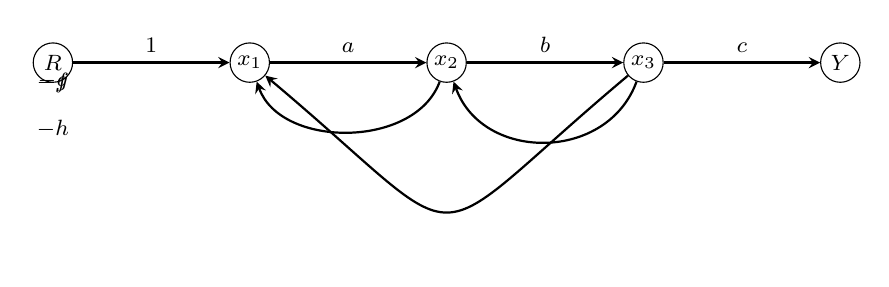
\begin{tikzpicture}[
    ctrlNode/.style={circle,draw=black,fill=white,minimum size=0.5cm,inner sep=0pt,font=\footnotesize},
    ctrlArrM/.style={->,>=stealth,thick},
    ctrlLabelM/.style={font=\footnotesize},
]
\node[ctrlNode] (ctrlR) at (0,0) {$R$};
\node[ctrlNode] (X1) at (2.5,0) {$x_1$};
\node[ctrlNode] (X2) at (5.0,0) {$x_2$};
\node[ctrlNode] (X3) at (7.5,0) {$x_3$};
\node[ctrlNode] (ctrlY) at (10,0) {$Y$};
\draw[ctrlArrM] (ctrlR) -- (X1) node[midway,above,ctrlLabelM] {$1$};
\draw[ctrlArrM] (X1) -- (X2) node[midway,above,ctrlLabelM] {$a$};
\draw[ctrlArrM] (X2) -- (X3) node[midway,above,ctrlLabelM] {$b$};
\draw[ctrlArrM] (X3) -- (ctrlY) node[midway,above,ctrlLabelM] {$c$};
% Feedback loop
\draw[ctrlArrM] (X2) to[out=250,in=290] (X1) node[midway,below,ctrlLabelM] {$-f$};
\draw[ctrlArrM] (X3) to[out=250,in=290,looseness=1.2] (X2) node[midway,below,ctrlLabelM] {$-g$};
\draw[ctrlArrM] (X3) to[out=220,in=320,looseness=2] (X1) node[pos=0.5,below=0.6cm,ctrlLabelM] {$-h$};
\end{tikzpicture}
\caption{信号流图示例}
\label{fig:sf-g}
\end{figure}

以图\ref{fig:sf-g}为例说明Mason公式的应用。前向通路：$P_1 = abc$（只有一条）。回路：$L_1 = -af$（$x_1\to x_2\to x_1$），$L_2 = -bg$（$x_2\to x_3\to x_2$），$L_3 = -ach$（$x_1\to x_2\to x_3\to x_1$）。互不接触回路对：$L_1$与$L_2$互不接触（无公共节点），乘积为$(-af)(-bg)=abfg$。

特征式：
\[
\Delta = 1 - (L_1+L_2+L_3) + (L_1L_2) = 1 + af + bg + ach + abfg
\]
所有回路均与$P_1$接触，故$\Delta_1 = 1$。由Mason公式：
\[
T = \frac{P_1\Delta_1}{\Delta} = \frac{abc}{1+af+bg+ach+abfg}
\]

\begin{example}
将框图\ref{fig:block-reduction}转换为信号流图并用Mason公式验证结果。

节点设为$R, x_1, x_2, x_3, Y$，其中$x_1$为$G_1$输出，$x_2$为$G_2$输出，$x_3$为$G_3$输出。前向通路：$P_1 = G_1G_2G_3$。回路：$L_1 = -G_2G_3H_2$，$L_2 = -G_1G_2G_3H_1$。$\Delta = 1 + G_2G_3H_2 + G_1G_2G_3H_1$，$\Delta_1 = 1$。
\[
T = \frac{G_1G_2G_3}{1 + G_2G_3H_2 + G_1G_2G_3H_1}
\]
与框图化简结果一致。
\end{example}

\section{典型系统的传递函数}

\subsection{闭环控制系统的基本传递函数}

考虑一般反馈控制系统（图\ref{fig:general-feedback}），定义以下传递函数：

\begin{figure}[H]
\centering
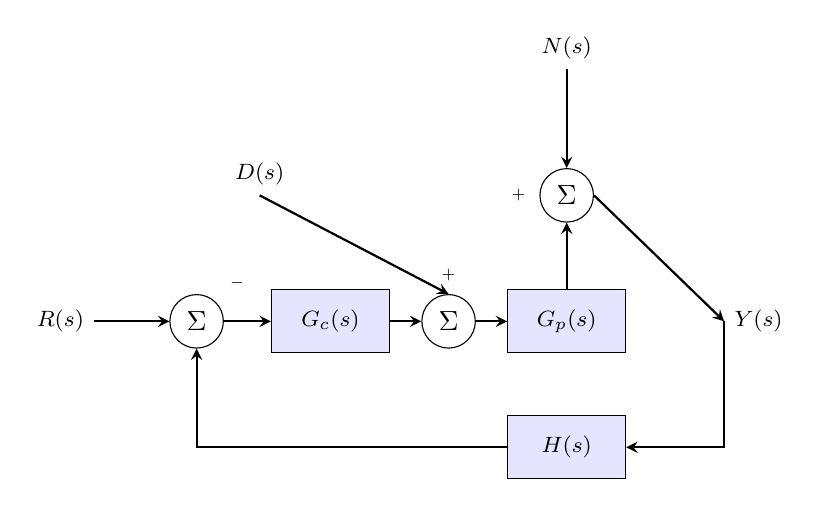
\begin{tikzpicture}[
    ctrlBkG/.style={rectangle,draw=black,fill=blue!10,minimum width=1.5cm,minimum height=0.8cm,font=\footnotesize},
    ctrlSmG/.style={circle,draw=black,minimum size=0.5cm},
    ctrlArrG/.style={->,>=stealth,thick},
]
\node[ctrlBkG] (GC) at (2.5,0) {$G_c(s)$};
\node[ctrlBkG] (GP) at (5.5,0) {$G_p(s)$};
\node[ctrlBkG] (HS) at (5.5,-1.6) {$H(s)$};
\node[ctrlSmG] (ctrlS) at (0.8,0) {$\Sigma$};
\node at (ctrlS.north east)[above right=0.05cm,font=\tiny] {$-$};
\node[ctrlSmG] (DS) at (4.0,0) {$\Sigma$};
\node at (DS.north)[above=0.05cm,font=\tiny] {$+$};
\node[ctrlSmG] (NS) at (5.5,1.6) {$\Sigma$};
\node at (NS.west)[left=0.05cm,font=\tiny] {$+$};
\draw[ctrlArrG] (-0.5,0) node[left,font=\footnotesize] {$R(s)$} -- (ctrlS);
\draw[ctrlArrG] (ctrlS) -- (GC);
\draw[ctrlArrG] (GC) -- (DS);
\draw[ctrlArrG] (DS) -- (GP);
\draw[ctrlArrG] (GP) -- (NS);
\draw[ctrlArrG] (NS.east) -- (7.5,0) node[right,font=\footnotesize] {$Y(s)$};
\draw[ctrlArrG] (7.5,0) -- (7.5,-1.6) -- (HS.east);
\draw[ctrlArrG] (HS.west) -- (0.8,-1.6) -- (ctrlS.south);
\draw[ctrlArrG] (1.6,1.6) node[above,font=\footnotesize] {$D(s)$} -- (DS.north);
\draw[ctrlArrG] (5.5,3.2) node[above,font=\footnotesize] {$N(s)$} -- (NS.north);
\end{tikzpicture}
\caption{考虑扰动$D(s)$和噪声$N(s)$的反馈控制系统}
\label{fig:general-feedback}
\end{figure}

\begin{enumerate}
\item \textbf{参考输入到输出的闭环传递函数}（$D=0, N=0$）：
\[
\Phi(s) = \frac{Y(s)}{R(s)} = \frac{G_c(s)G_p(s)}{1 + G_c(s)G_p(s)H(s)}
\]

\item \textbf{误差传递函数}（$D=0, N=0$）：
\[
\Phi_e(s) = \frac{E(s)}{R(s)} = \frac{1}{1 + G_c(s)G_p(s)H(s)}
\]

\item \textbf{扰动$D(s)$到输出$Y(s)$的传递函数}（$R=0, N=0$）：
\[
\Phi_d(s) = \frac{Y(s)}{D(s)} = \frac{G_p(s)}{1 + G_c(s)G_p(s)H(s)}
\]

\item \textbf{测量噪声$N(s)$到输出$Y(s)$的传递函数}（$R=0, D=0$）：
\[
\Phi_n(s) = \frac{Y(s)}{N(s)} = -\frac{G_c(s)G_p(s)H(s)}{1 + G_c(s)G_p(s)H(s)}
\]
\end{enumerate}

由叠加原理，系统总输出为：
\[
Y(s) = \Phi(s)R(s) + \Phi_d(s)D(s) + \Phi_n(s)N(s)
\]

\begin{remark}
四个传递函数具有{\heiti 相同的特征多项式}$1+G_cG_pH$——这正是一般反馈系统的核心特征：系统的稳定性、暂态行为由同一组闭环极点决定，与所考察的具体输入-输出通道无关。
\end{remark}

\subsection*{Python示例：传递函数建模与框图化简验证}

\begin{lstlisting}[language=Python]
import sympy as sp

# 定义符号
s = sp.symbols('s')
G1, G2, G3, H1, H2 = sp.symbols('G1 G2 G3 H1 H2')

# 方法1：逐步化简
# 最内环 G2-G3-H2
G23_inner = G2 / (1 + G2 * G3 * H2)
# 整个系统
T1 = sp.simplify(G1 * G23_inner * G3 / (1 + G1 * G23_inner * G3 * H1))
print("逐步化简结果:")
sp.pprint(T1)

# 方法2：Mason公式
Delta = 1 + G2*G3*H2 + G1*G2*G3*H1
P1 = G1*G2*G3
Delta1 = 1
T2 = sp.simplify(P1 * Delta1 / Delta)
print("\nMason公式结果:")
sp.pprint(T2)

# 验证等价性
print("\n两者相等:", sp.simplify(T1 - T2) == 0)
\end{lstlisting}

\begin{remark}
本章系统介绍了控制系统数学模型的建立方法。从微分方程到传递函数，从框图化简到Mason公式，核心思想始终是将复杂的物理系统抽象为简洁的数学描述。典型环节的传递函数是构建任何复杂系统的基本模块，框图化简和Mason公式则是处理多回路系统的工具——前者直观但步骤繁琐，后者简洁但需仔细识别回路和通路。在后续章节中，本章建立的数学模型将成为时域分析、根轨迹和频域分析的出发点。
\end{remark}
